\setcounter{chapter}{5}
\setcounter{rq}{1}


\chapter{Identifying Task-Relevant Text}
\label{ch:assisting}


% A developer can more effectively complete a software development task when automatically provided with text relevant to their task extracted from pertinent natural language artifacts and represented in a concise and thorough way.  

% \textbf{Thesis statement:} \textit{
%     Information relevant to a software development task can be automatically extracted from natural 
%     language software artifacts by interpreting the meaning, or semantics, of the text in these artifacts.
%     This task-relevant text assists a developer in effectively completing their software development task.
% }


Reviewing \textbf{thesis statement} to show chapter motivation.

\medskip
% \textbf{Thesis statement:} 
\textit{
    ``A developer can more effectively complete a software development task when provided
    with text that automatic techniques determine as relevant to the developer's task 
    according to the meaning, or semantics, of the text.''    
}

\medskip


Chapter needs to show that a semantic-based technique from previous chapter assists a 
developer effectively complete their task. Must define \textit{effectively}: 

\begin{itemize}
    \item correct: the solution for the task meets some correctness criteria, e.g., it meets expectations from a unit test
    \item complete: the solution meets some completeness criteria, e.g., it passes `\textit{all}' expected unit tests
\end{itemize}


This leads to a `within subjects' or `between subjects' evaluation where we assess whether 
a developer's solution is more correct or complete
 when assisted by a tool that embeds one semantic-based technique.

\begin{itemize}
\item independent variable: task done with or without tool
\item dependent variable(s): completeness and correctness of the task
\end{itemize}


\clearpage


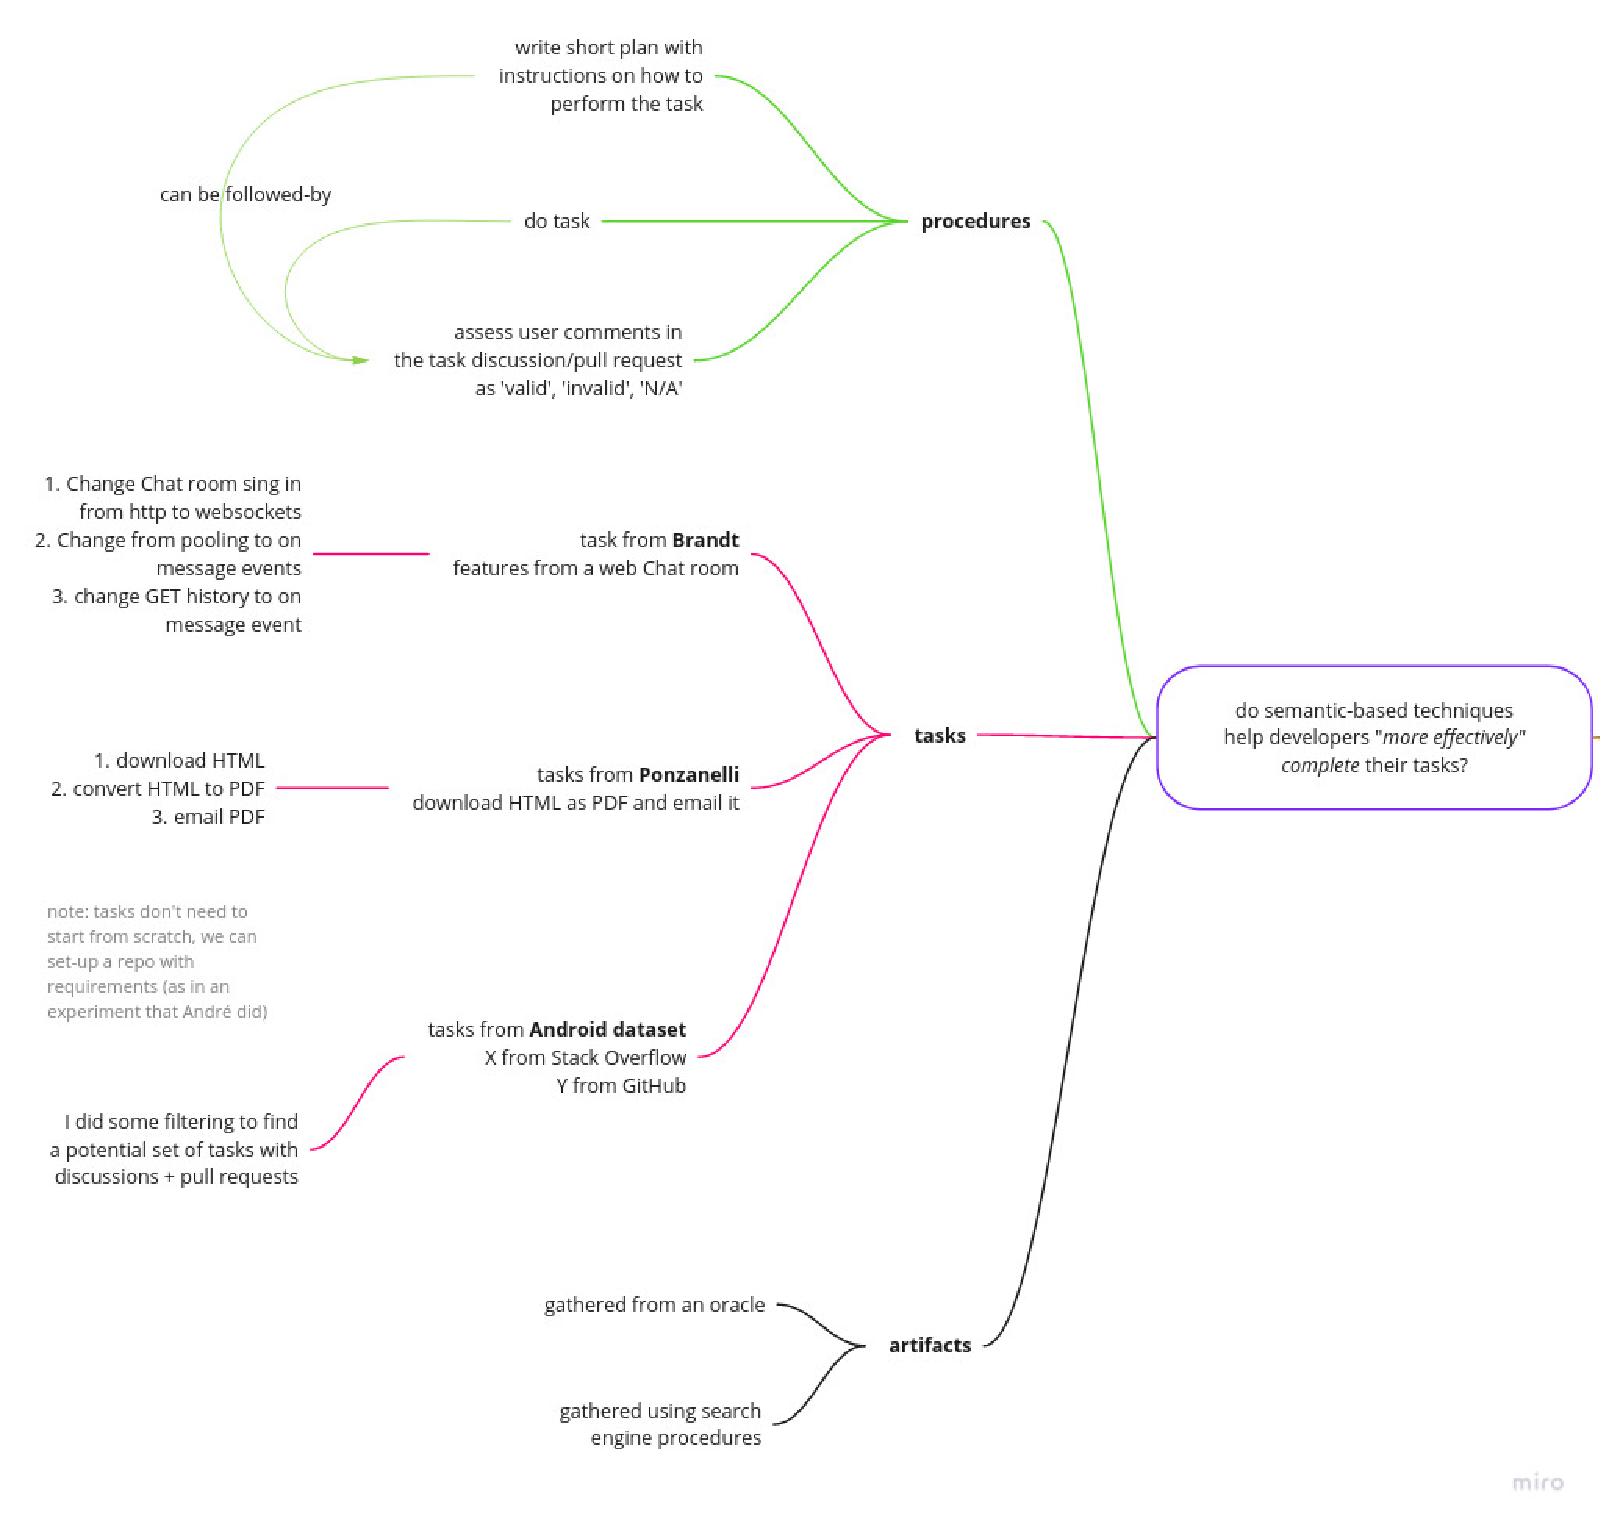
\includepdf[pages=-]{fig/cp6/ideas.pdf}


% \clearpage

\subsubsection{Brainstorm - A}

% \begin{small}
\begin{description}[leftmargin=\parindent, font=\normalfont\itshape]

    
    \item[procedures:] given a software task from a Stack Overflow post or a GitHub issue, write a short plan with instructions to solve the task

    
    \item[follow-up:] given user comments extracted from the Stack Overflow post or the GitHub issue, evaluate their correctness (whether the comment is correct or not)

    \item[tasks:] 5 random SO tasks and 5 random github tasks from Android
    
    \item[participants:] experienced developers
    
    \item[design:] between subjects. Independent variable is presence (or not) of the technique that highlights text that might assist in the task
    
    \item[measurement-1:] Likert scale on participant's confidence about the correctness of their answer
    
    \item[measurement-2:] If the assessment provided by a participant for each statement matches the ones of an oracle. To create the oracle:
    
        -- True statements are picked from the comment history on SO or GitHub
        
        -- False statements are created by picking a comment and modifying it
        
    \item[tooling:] fixed set of artifacts associated with each task. Highlights in each artifact are cached
    
    \item[pros:] easier to run online

        -- might be doable on MTurk, which increases participant pool

    \item[cons:]  if tasks are just to evaluate truthness, participants are more likely to just search for the bits that answer each statement

        -- participants do not get to perform the software task itself
\end{description}
% \end{small}

% \clearpage

\subsubsection{Brainstorm - B}

% \begin{small}
\begin{description}[leftmargin=\parindent, font=\normalfont\itshape]

    
    \item[procedures:] given a development task \& a maintenance task, provide a solution to the task

    
    \item[tasks:] 1 development task and 1 maintenance task. Each solvable in at most a 1 hour session
    
    -- development task: same as in~\cite{Ponzanelli2014b}---create a program that, given an URL of a webpage, an email address, and a subject for the email
    converts the HTML page into a PDF. 
    
    \textit{[this can be futher divided into smaller tasks, e.g. 1 task to download some url as a PDF and another to convert it into a PDF]}
    
    -- maintenance task: adapted from~\cite{Brandt2009a}---modify a chat room web application from HTTP to websockets \textit{[this can be futher divided into smaller tasks]}
    
    
    \item[participants:] experienced developers. Awarded an Amazon gift card as compensation
    
    \item[design:] within subjects. Independent variable is presence (or not) of the technique that highlights text that might assist in the task
    
    \item[measurement-1:] Likert scale on participant's confidence about the correctness of their answer
    
    \item[measurement-2:] Unit tests to assess the solution provided by a participant 
    
    \item[tooling:] some pseudo search engine that provides a set of URLs for each task. Highlights for each task-url are cached
    
    \item[pros:] more realistic and tasks were validated in related work

        -- unit tests give a better sense on how correct is a participant's solution

    \item[cons:]  harder to recruit participants

        -- participants do not get to perform the software task itself
\end{description}
% \end{small}



% \section{Summary}
\label{cp5:summary}



In this chapter, we introduced six semantic-based techniques 
that incorporate semantics of words and sentences
to identify task-relevant text across a range of natural language artifacts.
We compare our proposed techniques to a state-of-the-art technique, AnswerBot,
specific to Stack Overflow artifacts and 
we evaluate them using a dataset that comprises  50 software tasks about Android development for
which human annotators identified pertinent text per task across a variety of kinds of software
artifacts.
Evaluation results show that semantic-based techniques 
achieve recall comparable to AnswerBot, but without the need for artifact-specific data, 
and that some of our proposed techniques perform equivalently well across
multiple artifact types. 


